
\section{Syntactic arguments}\label{syntactic-sec}

Many proofs or refutations of implications (or equivalences) between two equational laws $E,E'$ can be obtained from the syntactic form of the equation.  We discuss some techniques here that were useful in the ETP.

\subsection{Simple rewrites}\label{rewrite-sec}

Many equational laws $E'$ can be formally deduced from a given law $E$ by applying the Lean `rw' tactic to rewrite $E'$ repeatedly by some forward or backward application of $E$ applied to arguments that match some portion of $E$.  For instance, the commutative law \eqref{eq43} clearly implies $\x \op (\y \op \z) \formaleq (\y \op \z) \op \x$ \eqref{eq4531}
by a single such rewrite.  A brute force application of such rewrite methods is already able to directly generate about $15,000$ such implications, including many equivalences to the singleton law \eqref{eq2} and the constant law \eqref{eq46}.  After applying transitive closure, this generates about four million further such implications.

A simple observation that already generates many equivalences is that any equation of the form $\x \formaleq f(\y,\z,\dots)$ necessarily is equivalent to the trivial law $\x \formaleq \y$; similarly, an equation of the form $f(\x,\y) \formaleq g(\z,\w,\dots)$ implies $f(\x,\y) \formaleq f(\x',\y')$; and so forth. \note{Give some stats on how effective this is.}

\subsection{Matching invariants}

Fix an alphabet $X$. A \emph{matching invariant} is an assignment $I \colon \Magma_X \to {\mathcal I}$ of an object $I(w) \in {\mathcal I}$ in some space ${\mathcal I}$ to each word $w \in \Magma_X$ with the property that if an equational law $w_1 \formaleq w_2$ has matching invariants $I(w_1)=I(w_2)$, then the same matching $I(w'_1) = I(w'_2)$ holds for any consequence $w'_1 \formaleq w'_2$.  In particular, if one law $I(w_1)=I(w_2)$ and $I(w'_1) \neq I(w'_2)$, then the law $w_1 \formaleq w_2$ does not imply the law $w'_1 \formaleq w'_2$.

A simple example of a matching invariant is the multiplicity $(n_x)_{x \in X}$ of variables of a word: if $w_1,w_2$ have all variables $x$ appear the same number of times $n_x$ in both words, then any rewriting of a word $w$ using the law $w_1 \formaleq w_2$ will preserve this property.  Hence, if $w'_1, w'_2$ do not have that each variable appear the same number of times in both words, then $w_1 \formaleq w_2$ cannot imply $w'_1 \formaleq w'_2$.  For instance, the commutative law \eqref{eq43} cannot imply the left-absorptive law \eqref{eq4}.

One source of matching invariants comes from the free magma $\Magma_{X,\Gamma}$ of a theory:

\begin{proposition}[Free magmas and matching invariants]\label{free-inv}  Let $\Gamma$ be a theory, and let $\iota_{X,\Gamma} \colon X \to \Magma_{X,\Gamma}$ be the map associated to the free magma $\Magma_{X,\Gamma}$ for that theory.  Then the map $I \colon \Magma_X \to \Magma_{X,\Gamma}$ defined by $I(w) \coloneqq \varphi_{\iota_{X,\Gamma}}(w)$ is an invariant.
\end{proposition}

\begin{proof}  Suppose that $w_1 \formaleq w_2$ entails $w'_1 \formaleq w'_2$, and that $I(w_1) = I(w_2)$.  For any $f \colon X \to \Magma_{X,\Gamma}$, the two maps $\varphi_f, \varphi_{f,\Gamma} \circ \varphi_{\iota_{X,\Gamma}} \colon \Magma_X \to \Magma_{X,\Gamma}$ are both homomorphisms that extend $f$, hence agree by the universal property of $\Magma_X$, as displayed by the following commutative diagram:
\[\begin{tikzcd}
	&& X \\
	\\
	{\Magma_X} && {\Magma_{X,\Gamma}} && {\Magma_{X,\Gamma}}
	\arrow[hook, from=1-3, to=3-1]
	\arrow["{\iota_{X,\Gamma}}"', from=1-3, to=3-3]
	\arrow["f", from=1-3, to=3-5]
	\arrow["{I = \varphi_{\iota_{X,\Gamma}}}", from=3-1, to=3-3]
	\arrow["{\varphi_f}"', curve={height=18pt}, from=3-1, to=3-5]
	\arrow["{\varphi_{f,\Gamma}}", from=3-3, to=3-5]
\end{tikzcd}\]
In particular, the hypothesis $I(w_1)=I(w_2)$ implies that $\varphi_f(w_1) = \varphi_f(w_2)$ for all $f \colon X \to \Magma_{X,\Gamma}$; that is to say, the magma $\Magma_{X,\Gamma}$ obeys the law $w_1 \formaleq w_2$, and hence also $w'_1 \formaleq w'_2$ by hypothesis.  In particular, $\varphi_{\iota_{X,\Gamma}}(w'_1) = \varphi_{\iota_{X,\Gamma}}(w'_2)$, which gives $I(w'_1) = I(w'_2)$ as required.
\end{proof}

\begin{example}  If we take $\Gamma = \{E4\}$ to be the theory of the left-absorptive law \eqref{eq4} as described in \Cref{left-absorb}, then the matching invariant $I(w)$ produced by \Cref{free-inv} is the left-most letter of the alphabet $X$ appearing in the word; for instance $I((\x \op \y) \op \z) = \x$.  Thus, for example, the left-absorptive law \eqref{eq4} cannot imply the right-absorptive law \eqref{eq5}.
\end{example}

\begin{example}  If we take $\Gamma = \{E43, E4512\}$ to be the theory of the commutative law \eqref{eq43} and the associative law \eqref{eq4512}, then by \Cref{semi-group}, the associated invariant $I(w) = \sum_{x \in X} n_x e_x$ is the formal sum of all the generators $e_x$ appearing in the word $w$, in the free abelian semigroup generated by those generators.  This recovers the preceding observation that the multiplicities $(n_x)_{x \in X}$ form a matching invariant.
\end{example}

\begin{example}  Let $n \geq 1$ be a positive integer, and consider the theory $\Gamma = \{E43, E4512, E_n\}$ consisting of the previous theory $\{E43, E4512\}$ together with the order-$n$ law $L_x^y x = y$.  One can check that the free magma $\Magma_{X,\Gamma}$ can be described as the free group of exponent $n$ with generators $e_x, x \in X$, with associated map $\iota_{X,\Gamma} \colon x \mapsto e_x$.  The associated matching invariant $I(w) = \sum_{x \in X} n_x e_x$ is essentially the multiplicities $(n_x \hbox{ mod } n)_{x \in X}$ modulo $n$, which gives a slightly stronger criterion than the preceding matching invariant for refuting implications.  For example, the cubic idempotent law $\x \formaleq (\x \op x) \op \x$ \eqref{eq23}
has matching invariants $e_x = 3e_x$ in the $n=2$ case, and hence does not imply the idempotent law $\x \formaleq \x \op \x$ \eqref{eq3} since $e_x \neq 2e_x$ in the $n=2$ case.
\end{example}

\note{Give some statistics on how many refutations can be established by these methods.}

\begin{remark}  One can also obtain matching invariants from the free objects associated to theories that involve additional operations beyond the magma operation $\op$, such as an identity element or an inverse operation.  We leave the precise generalization of \Cref{free-inv} to such theories to the interested reader.
\end{remark}

\subsection{Confluence}

We briefly recall the basics of rewrite theory necessary to our exposition, following mostly Baader and Nipkow \cite{traat}, and generally omitting proofs when they can be found there.

We first work in the abstract taking an arbitrary set $A$, with a given equivalence relation over it which we denote $\approx$. We consider a relation $R$ over $A$.

\begin{definition}
  We write $a \rightarrow b$ if $a\ R\ b$ holds in $A$, and say that $a$ \emph{rewrites to} (or \emph{reduces to}) $b$. We further define
  \begin{itemize}
    \item $\rightarrow^+$ as the transitive closure of $R$.
    \item $\rightarrow^*$ as the reflexive transitive closure of $R$.
    \item $\leftrightarrow^*$ as the reflexive transitive and symmetric closure of $R$.
  \end{itemize}
  We sometimes write $b\leftarrow a$, (resp. $b\ {}^*\leftarrow a$ etc) to mean $a\rightarrow b$ (resp. $a\rightarrow^*b$ etc), and chain notations, e.g. $b_1\leftarrow a\rightarrow b_2$.
\end{definition}

Note that $\leftrightarrow^*$ is an equivalence relation and the hope is for it to be equal to $\approx$, in order to deduce properties of the latter.

One should first note that if even $R$ is contained in $\approx$, then so are $\rightarrow^+, \rightarrow^*$ and $\leftrightarrow^*$ (as it is an equivalence relation), so we will focus on that case. Generally $a \rightarrow^* b$ can be seen as a way to \emph{compute} the $\approx$ relation, as it is directed, in a way to constrain our search space.

However, in general, we cannot deduce the converse, so it may be the case that $a\approx b$ but neither $a\rightarrow^*b$ nor $b\rightarrow^*a$ nor even is there a single $c$ such that $a\rightarrow^* c\ {}^*\leftarrow b$, as the number of ``left-right alternations'' may be arbitrarily large.

The following properties are going to be very useful to deduce exactly such a converse.

\begin{definition}
  We say that $R$ is \emph{Church-Rosser} if whenever $a\leftrightarrow^* b$, there exists some $c$ such that
  \[a\rightarrow^* c\ {}^*\leftarrow b\]
  We say that $R$ is \emph{confluent} if whenever $b_1\ {}^*\leftarrow a\rightarrow^* b_2$ there exists some $c$ such that $b_1\rightarrow^* c\ {}^*\leftarrow b_2$.

  We say that $R$ is \emph{locally confluent} if whenever $b_1\leftarrow a\rightarrow b_2$ there exists some $c$ such that $b_1\rightarrow^* c\ {}^*\leftarrow b_2$.

  We say that (an arbitrary) $a$ is in \emph{normal form} (or $a$ is a normal form) if there is no $a' \neq a$ such that $a \rightarrow a'$, and that $R$ is \emph{weakly normalizing} if for every $a$, there is some $a'$ such that $a\rightarrow^*a'$ and $a'$ is in normal form.

  We say that $R$ is \emph{strongly normalizing} if there are no infinite rewrite sequences $a_1\rightarrow a_2\rightarrow \ldots$. In particular, a strongly normalizing $R$ is also weakly normalizing.
\end{definition}

It turns out that if $R$ is strongly normalizing and Church-Rosser, and effective (we can ``compute'' with it) then the problem of equivalence is decidable! This is because of the following lemma.

\begin{lemma}
  If $R$ is Church-Rosser, then any normal form is \emph{unique}.
\end{lemma}

This means that, in this situation, $a$ and $b$ reduce to an identical normal form $c$ \emph{if and only if} $a\leftrightarrow^* b$! This means that we have the following algorithm to decide $a\leftrightarrow^* b$ (and therefore $a\approx b$ if these relations coincide):
\begin{enumerate}
  \item Repeatedly apply $R$ to $a$ and $b$ until normal forms $a'$ and $b'$ are found for them (this is possible because $R$ is strongly normalizing).
  \item Compare $a'$ and $b'$ for exact equality (sometimes called ``syntactic equality'').
  \item If $a' = b'$, we can conclude $a\leftrightarrow^* b$.
  \item If $a' \neq b'$ can can conclude that they are \emph{not} equivalent due to the lemma.
\end{enumerate}

Note that weak normalization does not change much here except at step 1, where we need to pick reductions which eventually bring the elements to normal forms.

The strategy is therefore, for a given $\approx$ to find an $R$ which is (strongly) normalizing and Church-Rosser, and such that $\leftrightarrow^*\ =\ \approx$. This is roughly the goal of the entire field of \emph{completion}. We call such an $R$ \emph{complete for} $\approx$.

The task is helped by the following facts, which we state here also without proof.

\begin{theorem}
  \begin{enumerate}
    \item $R$ is Church-Rosser iff it is confluent.
    \item (Newman's lemma) if $R$ is strongly normalizing, then $R$ is confluent iff it is locally confluent.
  \end{enumerate}
\end{theorem}

This strategy can be leveraged by looking at the particulars of the equivalence relation of interest, namely quantified equations over syntactic trees as in \Cref{abstract-nonsense-chapter}, and a theory $\Gamma$, which we will usually take to be finite (usually it will have a single equation!).

We will therefore consider relations over the set of elements of the free magma $M_{X}$, and the aim is to find a rewrite system $R$ is complete for $\formaleq$.

Certainly $\formaleq$ is closed over substitutions, and be a \emph{congruence}: if $a\formaleq a'$ and $b\formaleq b'$ under $\Gamma$, then $a\op b\formaleq a'\op b'$ under $\Gamma$ as well.

We therefore consider $R$ to be both closed under substitutions and a congruence. A convenient way to represent this is via a \emph{rewrite system}: simply a set of pairs of words $(l, r) \in M_{X}$ (we typically write $l\rightarrow r$) which represents the smallest congruence, closed by substitutions that contains those pairs.

Naturally, a set of laws $w \formaleq w'$ can be seen, given a choice of orientation (left-to-right or right-to-left) for each law as such a rewrite system. In this case, it is very clear that the reflexive transitive closure $\leftrightarrow^*$ recovers the original equational theory $\Gamma\models \cdot\formaleq\cdot$. However, it's clear that sometimes these systems will either be not strongly normalizing, or confluent, or both.

For example, it's clear that commutativity (the rule $x\cdot y\formaleq y\cdot x$ cannot possibly be oriented. Here is a non-confluent example:

\[ x \cdot (y \cdot z) \rightarrow y \]
We have $a\cdot (b \cdot (c \cdot d)) \rightarrow^* b$, but also $a\cdot (b\cdot (c\cdot d))\rightarrow^* a\cdot c$ for any $a, b, c, d$ (which are both in normal form).

Knuth and Bendix \cite{knuth-bendix} described a technique by which a theory or set of equations $\Gamma$ could be turned into a complete system. The crucial idea is the observation that the non-local-confluence of a rewrite system can be reduced to a finite (if the system is finite) set of ``worst offenders'' for confluence. If these pairs can be \emph{joined} (reduced to the same term) then the system is confluent. It is possible to compute such pairs.

The high-level idea is therefore to identify such pairs, and add them as an unoriented equation, to be oriented if possible, and repeating until no un-joinable pairs exist. If this procedure succeeds and terminates, the system is successfully completed, and as a result the theory $\Gamma$ is decidable, via the completed system as described above.

We use the intuitive notions of ``position in a word'' and ``word at a position $p$''. We denote by $w[w']_p$ the word $w$ with $w'$ inserted at position $p$.

\begin{definition}
  Given a rewrite system $R$ and two rules $\rho_1: l_1\rightarrow r_1$ and $\rho_2: l_2\rightarrow r_2$ in $R$, we say that $(t, u)$ is a \emph{critical pair} for $\rho_1$ and $\rho_2$ if there is some non-variable position $p$ in $l_1$ such that $l_2$ unifies with the term at that position. We denote by $\sigma$ the most general unifier thus obtained and have $t = r_1\sigma$ and $u = l_1\sigma[r_2\sigma]_p$
\end{definition}

Note that, in the above setting, $t\leftarrow l_1\sigma\rightarrow u$, giving us a candidate for non-local-confluence. The next lemma states that these candidates are the most general ones.

\begin{theorem}
  Given a rewrite system $R$, if for every critical pair $(t, u)$ of $R$, there is a term $v$ such that $t\rightarrow^* v\ {}^*\leftarrow u$, then $R$ is locally confluent.
\end{theorem}

Note that building critical pairs of a finite system is computable. Therefore the only step of the completion process which require genuine creativity is the choice of the orientation of the equations, along with the proof that that orientation is strongly normalizing.

We note that even in the event that such an orientation is not found, one can still partially apply the completion procedure, using any well-founded order on terms that is stable by substitution and congruence, to obtain a semi-decision procedure for equality. This process is sometimes called \emph{unfailing completion} and is at the core of the \emph{superposition calculus} used in Vampire.

\note{Define a confluent law and give some examples.}

\note{Define a complete rewriting system and give some examples.}

The associative and commutative laws, $x \op (y \op z) \sim (x \op y) \op z$ and $x \op y \sim y \op x$ both have confluent rewrite systems associated to them (by orienting the equations left-to-right). But it is easy to se that only the former has a complete rewrite system associated to it.

In addition it is easy to show, e.g. that $x \op (x \op x) \sim x$ has a natural orientation that is normalizing and such that the critical pairs are joinable, and hence is complete. This approach works for many rules.

It is easy to define a matching invariant for a complete system $R$ associated to $\Gamma$, by simply taking as model the elements of $\Magma_{X}$, the free magma without any relations, restricted to the elements $t \in \Magma_{X}$ that are irreducible under $R$. The interpretation function $\phi$ simply takes a term to its normal form (under $R$). The lemma above ensures that this is preserved under $\Gamma$.

\subsection{Unique factorization}

In general, the free magma $\Magma_{X,E}$ for a given equational law $E$, which we can canonically define as $\Magma_X / \sim_E$, is hard to describe explicitly; indeed, from the undecidability of implications between equational laws, such a magma cannot be computably described for arbitrary $E$.  Nevertheless, for some laws it is possible to obtain some partial understanding of $\Magma_{X,E}$ from a syntactic perspective.  For instance, if we can refute the equivalence $w'_1 \sim_E w'_2$ by constructing a counterexample magma $M$ that obeys $E$ but not $w'_1 \formaleq w'_2$, then this implies that the representatives $\iota_{X,E}(w'_1), \iota_{X,E}(w'_2)$ of  $w'_1, w'_2$ in $\Magma_{X,E}$ are distinct.

We illustrate this approach with equations $E$ of a left-absorptive form
\begin{equation}\label{left-absorptive}
\x \formaleq \x \op f(\x,\y,\z)
\end{equation}
for some word $f(\x,\y,\z)$, which imply the right-idempotent law \eqref{eq378}.

An illustrative example is the law \eqref{eq854} depicted in Figure \ref{fig:854}. Other examples are listed in \Cref{fig:854-like}.

\begin{figure}
  \centering
  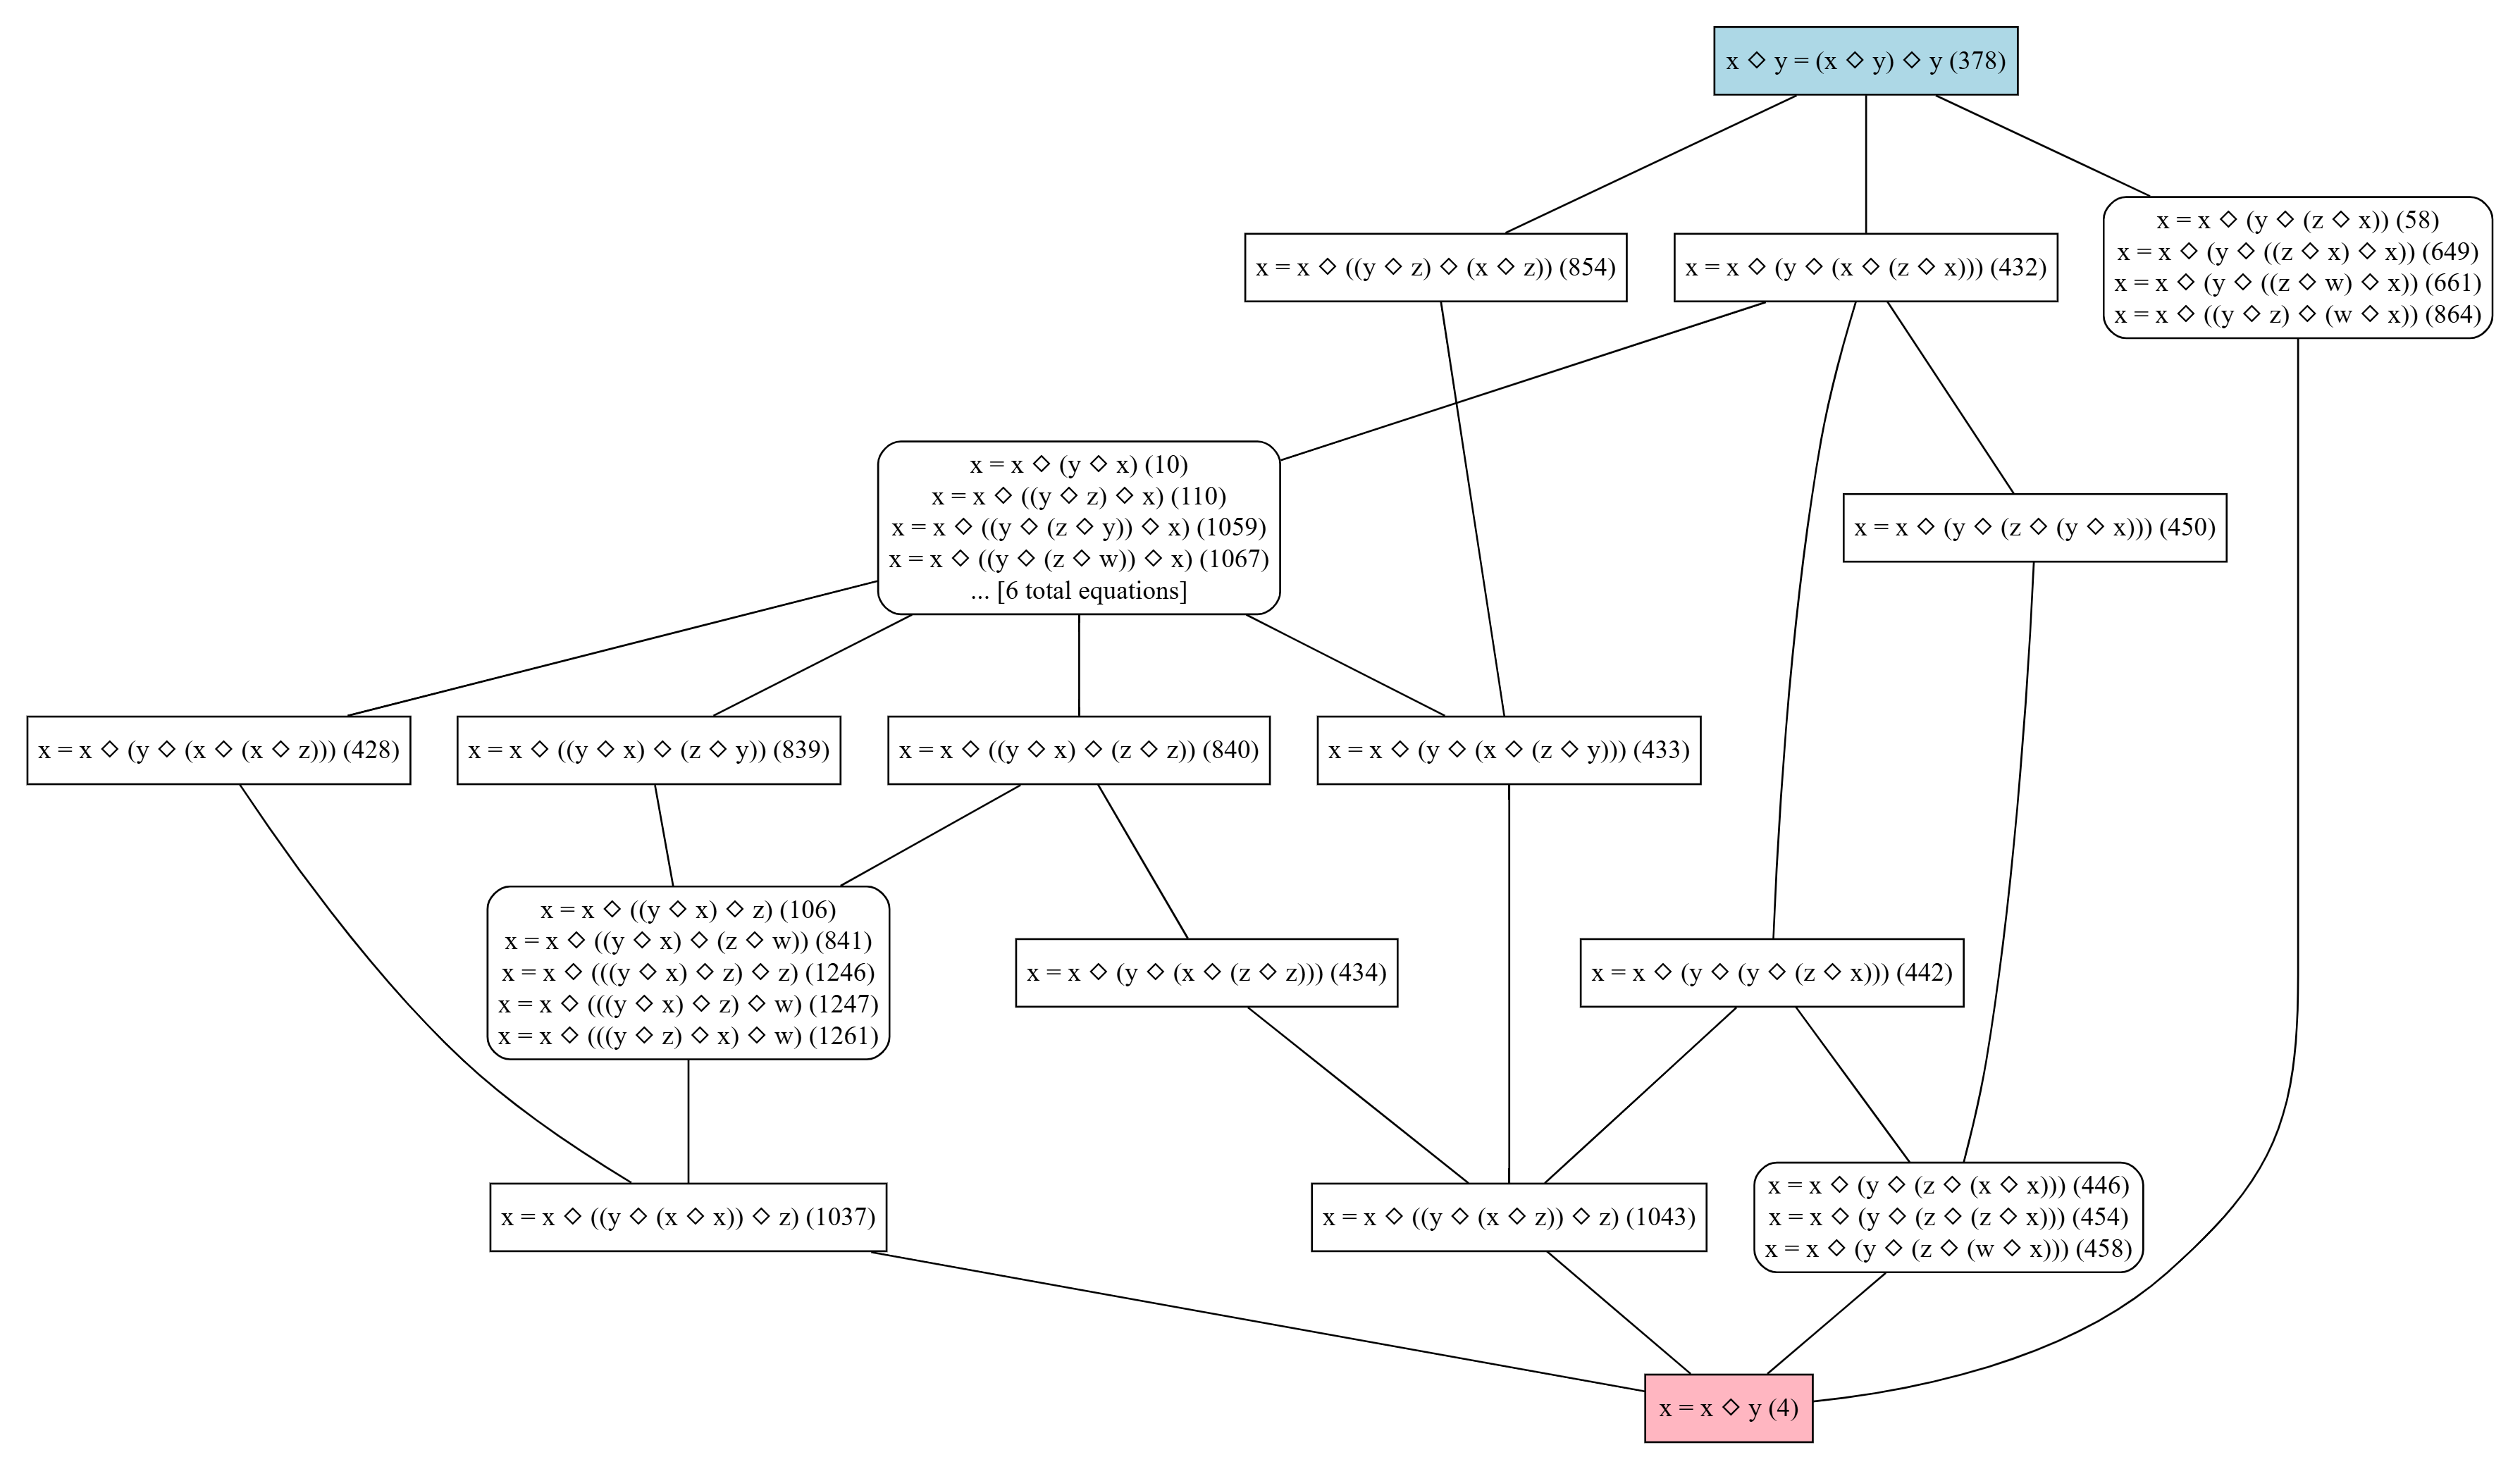
\includegraphics[width=0.85\textwidth]{854-like.png}
  \caption{Equations similar to \eqref{eq854} that are of the form \Cref{left-absorptive} (possibly involving a fourth indeterminate $\w$) and imply \eqref{eq378}.  For brevity, 70 equations equivalent to \eqref{eq4} have been omitted.}
  \label{fig:854-like}
  \end{figure}


\begin{lemma}\label{854} Equation \eqref{eq854} is of the form \Cref{left-absorptive} and implies \eqref{eq378}.
\end{lemma}

\begin{proof}  Clearly we have \Cref{left-absorptive} with $f(\x,\y,\z) \coloneqq (\y \op \z) \op (\x \op \z)$.  From \Cref{left-absorptive} we have in any magma obeying \eqref{eq854} that
$$x = x \op f(x,S^2 x,x) = x \op S(x \op S^2 x) = x \op S(x \op f(x,x,x)) = x \op Sx.$$
This implies from a further application of \Cref{left-absorptive} that
$$ y = y \op f(y,x,y) = (y \op Sy) \op ((x \op y) \op Sy) = f(x \op y, y, Sy)$$
and hence by \Cref{left-absorptive} again
$$ (x \op y) \op y = x \op y$$
giving \eqref{eq378}.
\end{proof}

Let $E$ be a law of the form \Cref{left-absorptive} that implies \eqref{eq378}. We define a directed graph $\to_E$ on words in $\Magma_X$ by declaring $w' \to_E w$ if $w \sim_E w'' \op w'$ for some $w' \in \Magma_X$.  By \eqref{eq378} (applied to the quotient magma $\Magma_{X,E} = \Magma_X/\sim_E$), this is equivalent to requiring that $w \sim_E w \op w'$. In particular, from \Cref{left-absorptive} we have $f(x,y,z) \to x$ for all $x,y,z$.  Furthermore, the relation $\to_E$ factors through $\sim_E$: if $w \sim_E \tilde w$ and $w' \sim_E \tilde w'$, then $w' \to_E w$ if and only if $\tilde w \to_E \tilde w$.

Call a word $w \in M_X$ \emph{irreducible} if it is not of the form $w = w_1 \op w_2$ with $w_2 \to_E w_1$.  We can partially understand the equivalence relation $\sim_E$ on irreducible words:

\begin{theorem}[Description of equivalence]\label{irred-desc}  Let $E$ be an equation of the form \Cref{left-absorptive}.  Let $w$ be an irreducible word, and let $w'$ be a word with $w \sim_E w'$.
  \begin{itemize}
    \item[(i)] If $w$ is a product $w = w_1 \op w_2$, then $w'$ takes the form
$$ w' = (((w'_1 \op w'_2) \op v_1) \op \dots \op v_n)$$
for some $w'_1 \sim_E w_1$, $w'_2 \sim_E w_2$, some $n \geq 0$, and some words $v_1, \dots, v_n$ such that for all $0 \leq i < n$, $v_{i+1}$ is of the form
$$ v_{i+1} \sim_E f(x_i,y_i,z_i)$$
for some $x_i, y_i, z_i$ with
$$ x_i \sim_E (((w'_1 \op w'_2) \op v_1) \op \dots \op v_i).$$
In particular, $v_{i+1} \to_E x_i$.
  \item[(ii)] Similarly, if $w \in X$ is a generator of $M_X$, then $w'$ takes the form
$$ w' = ((w \op v_1) \op \dots \op v_n)$$
for some $n \geq 0$, and some words $v_1, \dots, v_n$ such that for all $0 \leq i < n$, $v_{i+1}$ is of the form
$$ v_{i+1} \sim_E f(x_i,y_i,z_i)$$
for some $x_i, y_i, z_i$ with
$$ x_i \sim_E ((w \op v_1) \op \dots \op v_i).$$
In particular, $v_{i+1} \to_E x_i$.
\end{itemize}
Conversely, any word of the above forms is equivalent to $w$.
\end{theorem}

\begin{proof}  We just verify claim (i), as claim (ii) is similar.  The converse direction is clear from \Cref{left-absorptive} (after quotienting by $\sim_E$), so it suffices to prove the forward claim. By the Birkhoff completeness theorem, it suffices to prove that the class of words described by (i) is preserved by any term rewriting operation, in which a term in the word is replaced by an equivalent term using \Cref{left-absorptive}.  Clearly the term being rewritten is in $w'_1$ or $w'_2$ then the form of the word is preserved, and similarly if the term being rewritten is in one of the $v_i$.  The only remaining case is if we are rewriting a term of the form
$$ x_i = (((w'_1 \op w'_2) \op v_1) \op \dots \op v_i).$$
If $i>0$ we can rewrite this term down to $x_{i-1}$, and this still preserves the required form (decrementing $n$ by one).  If $i=0$ then we cannot perform such a rewriting because of the irreducibility of $w_1 \op w_2$ and hence $w'_1 \op w'_2$.  Finally, we can rewrite $x_i$ to $x_i \op v$ where $v$ is of the form
$$ v_i = f(x_i,y,z),$$
and after some relabeling we are again of the required form (now incrementing $n$ by one). This covers all possible term rewriting operations, giving the claim.
\end{proof}

Specializing to the case where $w,w'$ are both irreducible, we conclude

\begin{corollary}[Unique factorization]\label{unique factorization}  Two irreducible words $w, w'$ are equivalent if and only if they are either the same generator of $X$, or are of the form $w = w_1 \op w_2$, $w' = w'_1 \op w'_2$ with $w_1 \sim_E w'_1$ and $w_2 \sim_E w'_2$.
\end{corollary}

As an application of this corollary, we establish

\begin{proposition}[E854 does not imply E3316]\label{854-3316} Equation \eqref{eq854} does not imply \eqref{eq3316}.
\end{proposition}

\begin{proof}(Sketch)
  We work in the free group $\Magma_X$ on two generators $X = \{\x,\y\}$.  It suffices to show that
$$  \x \op \y \not \sim_{E854} \x \op (\y \op (\x \op \y)).$$
Suppose this were not the case, then by \Cref{unique factorization} one of the following statements must hold:
\begin{itemize}
\item[(i)] $y \to_{E854} x$.
\item[(ii)] $(y \op (x \op y)) \to_{E854} x$.
\item[(iii)] $y \op (x \op y) \sim_{E854} y$.
\end{itemize}
If (i) holds, then we have $x \op y = x$ must hold in $\Magma_X/\sim_E$, hence \eqref{eq854} would imply \eqref{eq4}.  However, it is possible to refute this implication by a finite counterexample.

Similarly, if (iii) held, then \eqref{eq854} would have to imply \eqref{eq10}, but this can also be refuted by a finite magma.

Finally, if (ii) held, then the claim
$$  x \op y \sim x \op (y \op (x \op y))$$
to refute simplifies to
$$  x \op y \sim x$$
and we are back to (i), which we already know not to be the case.
\end{proof}
